\documentclass[12pt,english]{article}
\usepackage{fontspec}
\setmainfont[Mapping=tex-text]{Arial}
\usepackage{geometry}
\geometry{verbose,tmargin=0.5in,bmargin=1in,lmargin=1in,rmargin=1in}
\usepackage{array}
\usepackage{graphicx}
\usepackage{setspace}

\makeatletter

%%%%%%%%%%%%%%%%%%%%%%%%%%%%%% LyX specific LaTeX commands.
%% Because html converters don't know tabularnewline
\providecommand{\tabularnewline}{\\}

%%%%%%%%%%%%%%%%%%%%%%%%%%%%%% User specified LaTeX commands.
\usepackage{titling}
\usepackage{lipsum}

\makeatother

\usepackage{minted}
\setminted{linenos=true, frame=single, escapeinside={!!}, tabsize=2, breaklines=true}
\usepackage{polyglossia}
\setdefaultlanguage[variant=american]{english}

\begin{document}

\pretitle{\noindent \Large{\textbf{NOAA Technical Memorandum NOS CS XX}}\\ \rule{\linewidth}{2pt} \begin{center}}
\date{\vspace{-5ex}}
\title{\begin{flushleft}\Large{\textbf{Tech Memo Template}}\end{flushleft}}

\maketitle

% it is important to define the author AFTER calling the first \maketitle, because the first title page should not have an author
\author{Author 1 ^{1,2} \and Author 2 ^{1,2} \and Author 3 ^{1,2} \and Author 4 ^2 \and Author 5 ^2}

\vfill{}

\large{Silver Spring, Maryland}

\large{\today}

\vfill{}


\includegraphics[width=0.25\textwidth]{images/usdoc_logo}

\vfill{}

\textbf{\Huge{noaa}} \textbf{National Oceanic and Atmospheric Administration}

\rule[0.5ex]{1\columnwidth}{2pt}

\textbf{U.S. DEPARTMENT OF COMMERCE}

\textbf{National Ocean Service}

\textbf{Coast Survey Development Laboratory}

% it is important to clear the page style right before the new page in order to clear the page number from the first page 
\thispagestyle{empty}

\newpage{}

\vspace*{\fill}

\begin{center}
\textbf{Office of Coast Survey}

\textbf{National Ocean Service}

\textbf{National Oceanic and Atmospheric Administration}

\textbf{U.S. Department of Commerce}
\end{center}

\medskip{}

\noindent \textbf{The Office of Coast Survey (OCS) is the Nation’s only official chartmaker. As the oldest United States scientific organization, dating from 1807, this office has a long history. Today it promotes safe navigation by managing the National Oceanic and Atmospheric Administration’s (NOAA) nautical chart and oceanographic data collection and information programs.}

\medskip{}

\noindent \textbf{There are four components of OCS:}
\begin{enumerate}
\item \textbf{The Coast Survey Development Laboratory develops new and efficient techniques to accomplish Coast Survey missions and to produce new and improved products and services for the maritime community and other coastal users.}
\item \textbf{The Marine Chart Division acquires marine navigational data to construct and maintain nautical charts, Coast Pilots, and related marine products for the United States.}
\item \textbf{The Hydrographic Surveys Division directs programs for ship and shore-based hydrographic survey units and conducts general hydrographic survey operations.}
\item \textbf{The Navigational Services Division is the focal point for Coast Survey customer service activities, concentrating predominately on charting issues, fast-response hydrographic surveys, and Coast Pilot updates.}
\end{enumerate}

\vspace*{\fill}

\thispagestyle{empty}

\newpage{}

\pagenumbering{roman}
\setcounter{page}{1}

\maketitle

\medskip{}

\textbf{\scriptsize{1. Office of Coast Survey, Coast Survey Development Laboratory, Silver Spring, Maryland}}

\textbf{\scriptsize{2. University Corporation for Atmospheric Research, Boulder, Colorado}}

\vfill{}

\textbf{\large{\today}}

\vfill{}


\includegraphics[width=0.22\textwidth]{images/noaa_logo}

\vfill{}

\textbf{\Huge{noaa}} \textbf{National Oceanic and Atmospheric Administration}

\rule[0.5ex]{1\columnwidth}{2pt}

\medskip{}

\begin{tabular*}{1\textwidth}{@{\extracolsep{\fill}}>{\raggedright}b{0.33\textwidth}>{\raggedright}b{0.33\textwidth}>{\raggedright}b{0.33\textwidth}}

\noindent \textbf{\footnotesize{U. S. DEPARTMENT OF COMMERCE}} & \noindent \textbf{\footnotesize{Oceans and Atmosphere}} & \noindent \textbf{\footnotesize{National Ocean Service}}
\tabularnewline
\noindent \textbf{\footnotesize{Gina Raimondo}} & \noindent \textbf{\footnotesize{Richard Spinrad}} & \noindent \textbf{\footnotesize{Nicole LeBoeuf}}
\tabularnewline
\noindent \textbf{\footnotesize{Secretary}} & \noindent \textbf{\footnotesize{Under Secretary}} & \noindent \textbf{\footnotesize{Assistant Administrator}}
\tabularnewline
\end{tabular*}

\medskip{}

\begin{tabular*}{1\textwidth}{@{\extracolsep{\fill}}>{\raggedright}p{0.5\textwidth}>{\raggedright}p{0.5\textwidth}}
\textbf{\footnotesize{Office of Coast Survey}} & \textbf{\footnotesize{Coast Survey Development Laboratory}}
\tabularnewline
\textbf{\footnotesize{Captain Benjamin Evans}} & \textbf{\footnotesize{Shachak Pe’eri}}
\tabularnewline
\textbf{\footnotesize{Director}} & \textbf{\footnotesize{Division Chief}}
\tabularnewline
\end{tabular*}

\newpage{}

\vspace*{\fill}

\begin{center}
\textbf{\large{NOTICE}}
\end{center}

\vspace*{\bigskipamount}

\noindent \textbf{Mention of a commercial company or product does not constitute an endorsement by NOAA. Use for publicity or advertising purposes of information from this publication concerning proprietary products or the tests of such products is not authorized.}

\vspace*{\fill}

\newpage{}

\tableofcontents{}

\listoffigures

\newpage{}

\begin{abstract}
\lipsum[1] \cite{Taguchi2014}
\end{abstract}

\paragraph{Key Words}

key, words

\newpage ~\newpage{}

\pagenumbering{arabic}
\setcounter{page}{1}

\section{Introduction}

\lipsum[1] \cite{Egbert2002}

\lipsum[1-3]

\begin{figure}
    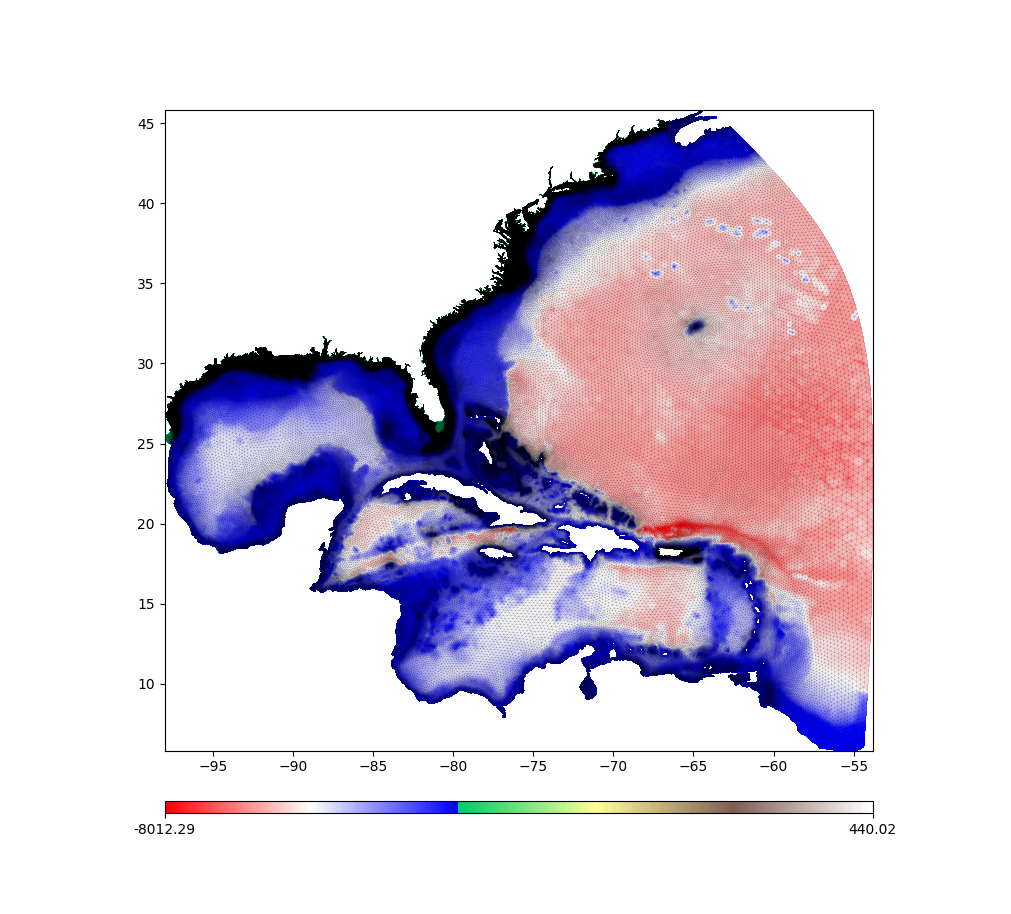
\includegraphics[width=\textwidth, keepaspectratio]{images/hsofs_mesh.png}
    \caption{HSOFS mesh}
    \label{fig:hsofs_mesh}
\end{figure}

\lipsum[1]

\section{Methodology}

Figure \ref{fig:hsofs_mesh} \lipsum[1-4]

\section{Results}

\lipsum[1-4]

\section{Analysis}

\lipsum[1-5]

\section{Discussion}

\lipsum[1-3]

\newpage{}

\section{Acknowledgments}

\lipsum[1] 

\bibliographystyle{plain}
\addcontentsline{toc}{section}{\refname}\bibliography{references}

\end{document}
